\documentclass[10pt]{beamer}

\usetheme{glasgow}

\usepackage{booktabs}
\usepackage[scale=2]{ccicons}
\usepackage{minted}
\usepackage{bookmark}
\usepackage[style=verbose]{biblatex}
\renewcommand{\footnotesize}{\fontsize{5pt}{7pt}\selectfont}
% \usepackage{filecontents}% to embed the file `myreferences.bib` in your `.tex` file
% \begin{filecontents*}[noheader]{references.bib}
%     @book{rappaport_millimeter_2015,
% 	address = {Upper Saddle River, NJ},
% 	title = {Millimeter wave wireless communications},
% 	isbn = {978-0-13-217228-8},
% 	publisher = {Prentice Hall},
% 	author = {Rappaport, Theodore S. and Heath, Robert W. and Daniels, Robert C. and Murdock, James N.},
% 	year = {2015},
% 	keywords = {Millimeter wave communication systems, Wireless communication systems}
% }

% \addbibresource{references.bib}


% \usepackage[noadjust]{cite}
\usepgfplotslibrary{dateplot}

\usemintedstyle{trac}

% ($ (A)!r!(B) $) the location of images to be used
\graphicspath{{src/}}

%% Customisation
% \newcommand{\V}[1]{\v} % vectors \v{c}
% \renewcommand{\v}[1]{\mathbf{#1}} % vectors
\newcommand{\ti}[1]{\tilde{#1}} % spectral representation
\newcommand{\tnsr}[1]{\underline{\underline{#1}}}

% Symbols
\renewcommand{\O}{\omega}  % omega
\newcommand{\E}{\varepsilon}  % epsilon
\renewcommand{\u}{\mu}  % mu
\newcommand{\p}{\rho}  % rho
\newcommand{\x}{\times}  % times
\renewcommand{\inf}{\infty}  % infinity
\newcommand{\infint}{\int\limits_{-\inf}^\inf} % integral by R
\newcommand{\e}{\mathrm{e}} % Straight-up exponential
\renewcommand{\j}{{j}\mkern1mu} % Straight-up exponential
\newcommand{\iu}{\mathrm{i}\mkern1mu}

\newcommand\ddfrac[2]{\frac{\displaystyle #1}{\displaystyle #2}}

\usepackage{animate}



%     % Define a the counter cnt. Used to identify files generated for use
% % with Gnuplot.
% \newcounter{cnt}
% \setcounter{cnt}{0}

% % Macro for drawing one frame of the F-distribution animation.
% \newcommand{\fdst}[4]{%
%     % shade the critical region tail
%     \draw[fill,orange]  (#1,0) -- plot[id=5\thecnt,domain=#1:5.5,samples=50]
%         function {#4*(x**(0.5*#2-1))*((1+#2*x/#3)**(-0.5*#2-0.5*#3))}
%             -- (5.5,0) -- cycle;

%     % draw the F distribution curve
%     \draw[color=blue!50!black,thick]
%         plot[id=f4\thecnt,smooth,domain=0:5.5,samples=100]
%         function {#4*(x**(0.5*#2-1))*((1+#2*x/#3)**(-0.5*#2-0.5*#3))};

%     % draw the F axis
%     \draw[->] (0,0) -- (6,0) node[right] {$F$};
%     % label the critical region boundary
%     \draw (#1,0) -- (#1,-0.02) node[below] {$#1$};
%     % label 0
%     \draw (0,0) -- (0,-0.02) node[below] {$0$};

%     % add some lables for degrees of freedom and alpha level
%     \draw (2,0.5) node[right] {$df_1 = #2$};
%     \draw (2,0.4) node[right] {$df_2 = #3$};
%     \draw (2,0.3) node[right] {$\alpha = 0.10$};

%     % draw the y axis
%     \draw[very thin,->] (0,0) -- (0,0.8);
% }


\title{High Frequency Communication Systems}
\subtitle{Lecture 10}
\date{Spring 2021}
\author{Hasan T Abbas \& Qammer H Abbasi}
% \institute{}





\begin{document}

\maketitle

%%%%%%%%%%%%%%%%%%%%%%%%%%%%%%%%%%%%%%%%%%
%%%%%%%%%%%%%%%%%%%%%%%%%%%%%%%%%%%%%%%%%%
%%%%%%%%%%%%%%%%%%%%%%%%%%%%%%%%%%%%%%%%%%
\begin{frame}[fragile]
    \frametitle{Lecture Outline}
    \begin{outline}[itemize]
        \1 mmWave Communications
        \1 mmWave Antennas
        \1 mmWave Beamforming Algorithms
    \end{outline}
\end{frame}
%%%%%%%%%%%%%%%%%%%%%%%%%%%%%%%%%%%%%%%%%%
%%%%%%%%%%%%%%%%%%%%%%%%%%%%%%%%%%%%%%%%%%
%%%%%%%%%%%%%%%%%%%%%%%%%%%%%%%%%%%%%%%%%%

\section{mmWave Communications}


\begin{frame}
    \frametitle{mmWave Communications}

    \begin{figure}[h!]
        \centering
        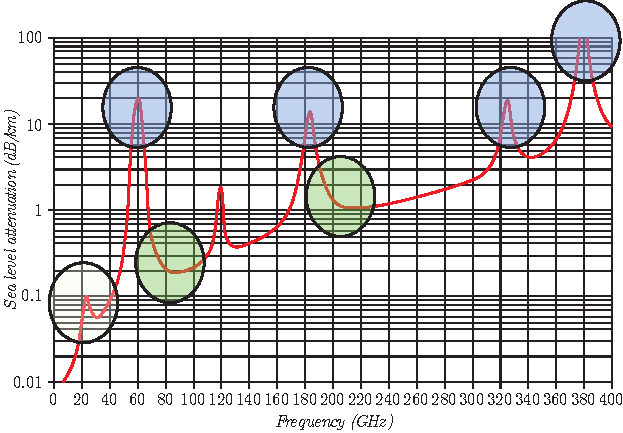
\includegraphics[width=.9\textwidth]{atmosphere.pdf}
        \caption{EM wave attenuation due to \ch{O2} molecules in air in the mmWave spectrum. \tiny{[T. S. Rappaport \textit{et al},  Proceedings of the IEEE, vol. 99, no. 8, pp. 1390-1436, 2011.]}}
    \end{figure}

\end{frame}

\begin{frame}
    \frametitle{EM wave propagation at mmWave frequencies}
    \normalsize
    \begin{outline}
        \1 $\lambda$ at mmWave becomes so small that the \ch{O2} and \ch{H2O} molecules in the air severely affect the wave propagation
        \1 Besides this, we have the effects of weather such as rain, fog etc.
        \2 The wave is also attenuated due to distance and other obstacles
        \1 \textcolor{red}{We need to design antennas that perform effective communications.}
    \end{outline}
\end{frame}

\begin{frame}
    \frametitle{mmWave Communications}
    \begin{columns}[T]
        \normalsize
        \begin{column}{.6\textwidth}
            \begin{outline}
                \1 mmWave signals have extremely short wavelengths ($\lambda = \SI{10.7}{\mm}$ at $\SI{28}{\GHz}$, $\lambda = \SI{5}{\mm}$ at $\SI{60}{\GHz}$)
                \1 As a result, objects that would scatter EM waves may now act as \textit{reflectors}.
                \2 Significantly higher multipath effects at mmWave as compared to microwave systems
                \1 These small dimensions enable extremely integrated and physically small antennas
                \2 In-package and on-chip antennas
                \2 We can make the antennas with the same fabrication process as the rest of the IC
            \end{outline}
        \end{column}
        \begin{column}{.4\textwidth}
            \scriptsize
            \begin{figure}[T!]
                \centering
                \subfloat[]{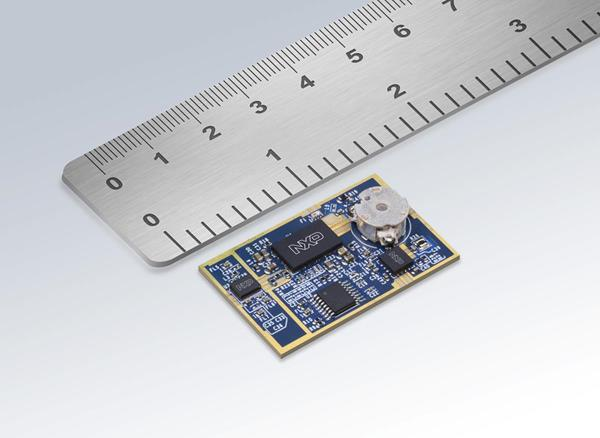
\includegraphics[width=.5\textwidth]{mMIMO-inner-board-ruler_HR.jpeg}
                    \label{fig:NXP_5G_chip}} \\
                \subfloat[]{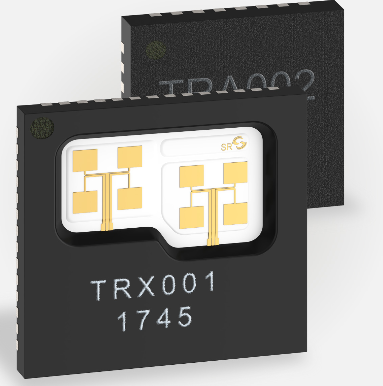
\includegraphics[width=.5\textwidth]{TRX120_001.png}
                    \label{fig:TRX_Silicon Radar}}
                \caption{\scriptsize An on-chip \SIrange{3}{5}{\GHz} and a  \SI{120}{\GHz} antenna in package ( \SI{8}{\mm} by \SI{8}{\mm}) (\textcopyright NXP Semiconductors, Silicon Radar).}
                \label{fig:antenna_on_chip}
            \end{figure}
        \end{column}
    \end{columns}
\end{frame}

\begin{frame}
    \frametitle{mmWave Propagation}

    \begin{outline}
        \1 The wave propagation can be modelled macroscopically (\textit{large-scale channel effects}) or microscopically (\textit{small-scale channel effects}
        )
        \1 Lets start with the \textit{Friis} transmission equation:
    \end{outline}

    \begin{align*}
        P_{\text{Rx}} {}= & \frac{P_{\text{Tx}} \mathrm{Gain}_{\text{Tx}}  \mathrm{Gain}_{\text{Rx}}}{\text{Loss Factor}} \left(\frac{\lambda}{4 \pi D}\right)^2
    \end{align*}

    \begin{figure}[h!]
        \centering
        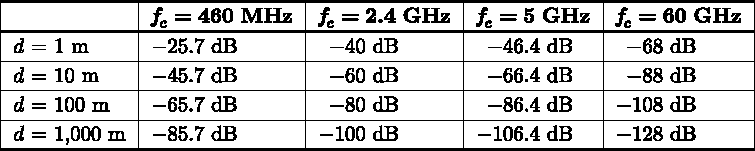
\includegraphics[width=0.75\textwidth]{table.pdf}
        \caption{Freespace Path Loss at different frequencies.}
    \end{figure}

\end{frame}



\begin{frame}
    \frametitle{Revisiting Antenna Gain}

    From previous lectures, the antenna gain is:
    \begin{align*}
        \mathrm{Gain}_{\max} {}= & e_{\max} A_{\max} \frac{4 \pi}{\lambda^{2}}
    \end{align*}
    We typically treat $A_{\max} \propto D^2$.    For a uniform linear array of $N$ elements,
    \begin{align*}
        D_{\text{array}} {}= & N \times D_{\text{element}}
    \end{align*}
    For a two-dimensional array, the gain therefore, becomes even higher,
    \begin{align*}
        \mathrm{Gain}_{\max} \propto \frac{4 \pi D_{\text{array}}^{2}}{\lambda^{2}}
    \end{align*}
    \begin{tcolorbox}[colback=blue!5]
        \begin{align*}
            P_{\text{Rx}}=\frac{P_{\text{Tx}} e_{\text{Tx}} e_{\text{Rx}}\left(D_{\text{Rx}} D_{\text{Tx}}\right)^{2}}{L(\lambda d)^{2}}
        \end{align*}
    \end{tcolorbox}
\end{frame}

\begin{frame}
    \frametitle{Some Important Observations}
    \begin{outline}
        \1 As frequency increases, we can stack more antenna elements in an array within a given size
        \2 Results in increased gain
        \1 The Tx and Rx antennas become highly directional
        \2 The steering of the beams becomes an altogether new topic of research
        \2 The path loss can be overcome
        \1 For a given gain, the effective area is proportional to $1/f^2$
        \1 However, the antenna efficiency typically decreases as we go up in frequency
    \end{outline}
\end{frame}


\begin{frame}
    \frametitle{Bandwidth and Power}

    According to the famous \textit{Shannon} capacity theorem, a wireless channel capacity, $C$ for a signal with power $P$ is,
    \begin{align*}
        C {}= & \text{BW} \log _{2}\left(1+\frac{P}{\text{BW} \, N_0}\right)
    \end{align*}
    where, $BW$ is the signal bandwidth, and $N_0$ is the noise spectral density.

    \begin{outline}
        \1 For a given power $P_0$, the capacity is an increasing function of $\text{BW}$.
        \1 However, we approach a limit,
    \end{outline}
    \begin{align*}
        \lim_{\text{BW} \rightarrow \infty} \text{BW} \log_{2}\left(1+\frac{P_0}{\text{BW} \,  N_{0}}\right) {}= & \frac{P_0}{\log (2) N_{0}}
    \end{align*}
\end{frame}

\begin{frame}
    \frametitle{Bandwidth and Power}
    We can only ever so get some bandwidth benefits out of a mmWave system.
    \begin{figure}[htbp]
        \centering
        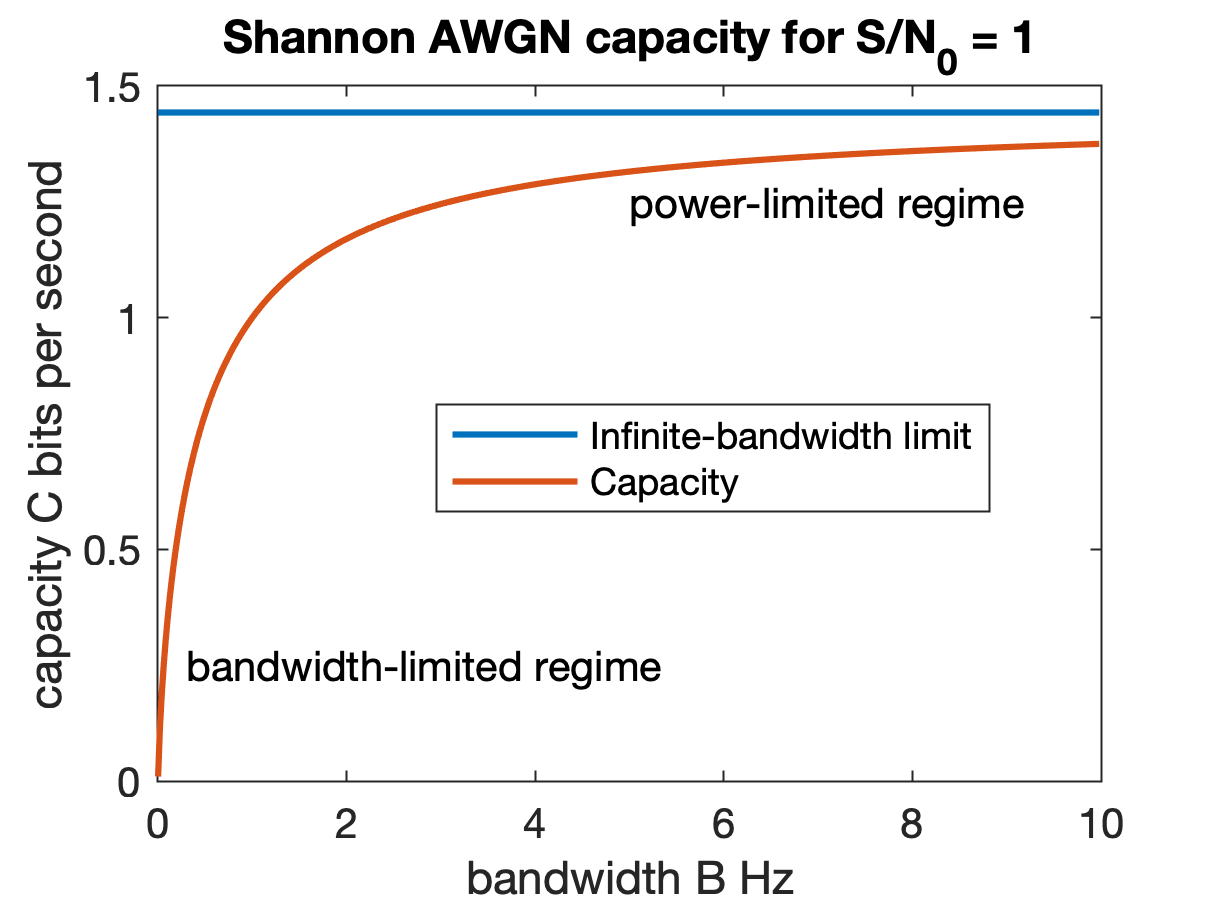
\includegraphics[width=.5\textwidth]{Channel_Capacity_with_Power-_and_Bandwidth-Limited_Regimes.png}
    \end{figure}
    \begin{tcolorbox}[colback=blue!5]
        For mmWave systems, we need to increase the power (\textit{gain}) to get a similar network performance.
    \end{tcolorbox}
\end{frame}


\begin{frame}
    \frametitle{Example - Finding the Number of Antennas}
    Consider, we want to have the same quality of service (i.e. same link budget) in the scenario below. What is the approximate number of antenna elements required in the mmWave case?

    Treat the antennas as ideal with the distance from the transmitter and similar efficiencies.

    \begin{figure}[h!]
        \centering
        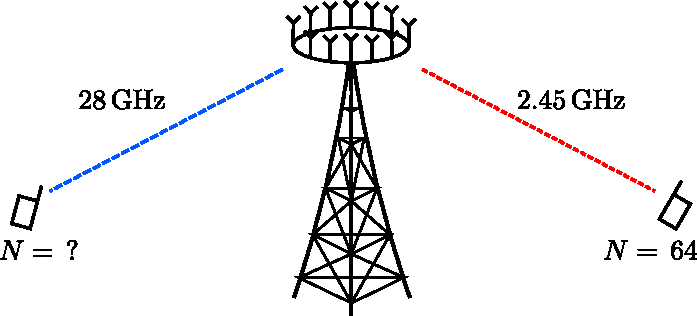
\includegraphics[width=.75\textwidth]{example_antenna.pdf}
    \end{figure}
\end{frame}

% \begin{frame}
%     \frametitle{Example - Solution}

%     From the \textit{Friis} formula, we can estimate the link budget. We would like to have the same power received in both cases.

%     An approximate value, discounting the efficiencies, interference and noise can be written as:
%     \begin{align*}
%         N_2 \approx \left(\frac{f_2}{f_1}\right)^2 N_1 \\
%         N_2 \approx 136.11 \times 64
%     \end{align*}

%     We need $\approx 136$ times more antennas to maintain the link budget!
% \end{frame}

\section{mmWave Antennas}

\begin{frame}
    \frametitle{mmWave Antennas}

    \begin{outline}
        \1 So far, we have considered an ideal scenario where we ignored all the factors that affect antenna performance
        \2 In reality, mmWave antennas are in-efficient
        \2 Feeding networks become complex due to the large number of array elements
        \1 With good designs, we can achieve antenna efficiency up to \SI{80}{\percent}
        \1 Mainly there are two types of designs, \textit{on-chip} and \textit{in-package} antennas
    \end{outline}
\end{frame}

\begin{frame}
    \frametitle{On-chip Antennas}
    \begin{columns}[T]
        \begin{column}{.5\textwidth}
            \begin{outline}
                \small
                \1 The biggest motivation behind the use of on-chip antennas is the low-cost and integration with the rest of electronics
                \1 We can achieve gain up to \SI{30}{\dB} and antenna efficiency over \SI{85}{\percent}
                \1 There are four design challenges that one has to consider
                \2 Generation of surface waves
                \2 Direction of antenna radiation
                \2 Substrate loss
                \2 Resonant frequency of the substrate
                \1 As the antenna may be surrounded by nearby metal vias, we need to consider coupling effects.
            \end{outline}
        \end{column}
        \begin{column}{.5\textwidth}
            \begin{figure}[T!]
                \centering
                \subfloat[]{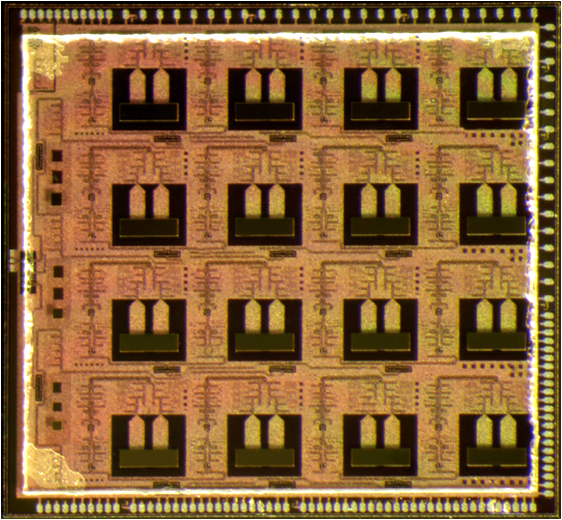
\includegraphics[width=.75\textwidth]{30-researchersd.jpeg}
                    \label{fig:on_chip}} \\
                \subfloat[]{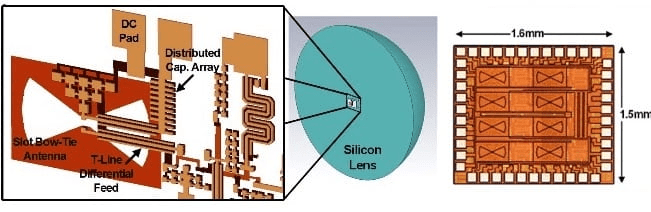
\includegraphics[width=.75\textwidth]{image.png}
                    \label{fig:antenna_on_chip}}
            \end{figure}
        \end{column}
    \end{columns}
\end{frame}

\begin{frame}
    \frametitle{On-chip Antennas - Surface Wave Generation}
    \begin{columns}[T]
        \begin{column}{.5\textwidth}
            \begin{outline}
                \1 The nature of the structure supports the unwanted generation and radiation of surface waves
                \1 Surface waves travel along the axis of the substrate
                \2 They reduce the efficiency
                \2 Increase the coupling between adjacent structures
                \1 \textcolor{red}{As a remedy, we can increase the substrate thickness to suppress the surface waves}
                \2 However, this has detrimental consequences on antenna efficiency
            \end{outline}
        \end{column}
        \begin{column}{.5\textwidth}
            \begin{figure}[T!]
                \centering
                \subfloat[]{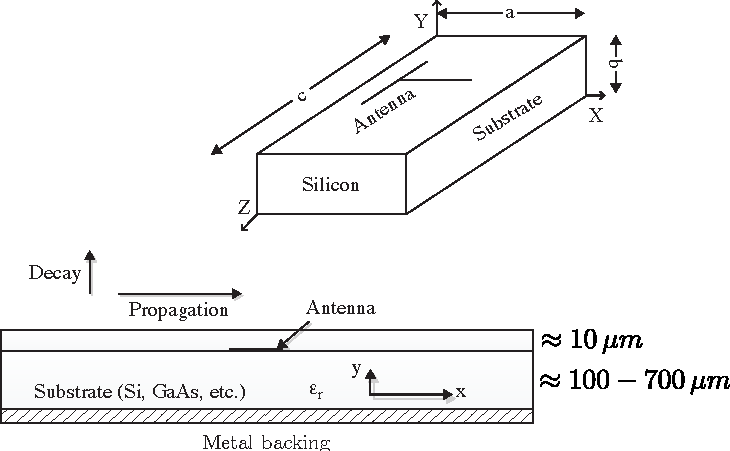
\includegraphics[width=.75\textwidth]{onchipantennas.pdf}
                    \label{fig:on_chip}} \\
                \subfloat[]{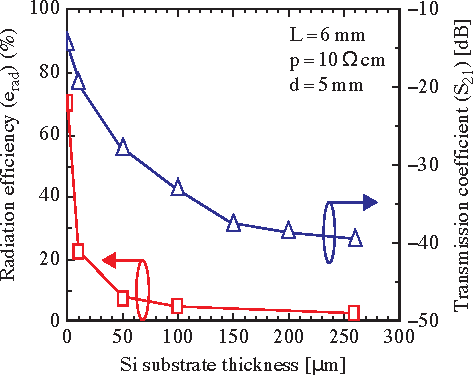
\includegraphics[width=.9\textwidth]{substrate_thickness.pdf}
                    \label{fig:antenna_on_chip}}
            \end{figure}
        \end{column}
    \end{columns}
\end{frame}

\begin{frame}
    \frametitle{On-chip antennas - Direction of radiation}
    \begin{columns}[T]
        \begin{column}{.5\textwidth}
            \begin{outline}
                \1 Due to the high dielectic permittivity of \ch{Si} ($\E = 11.7$), the direction of radiation is \textcolor{red}{into} the substrate rather than out.
                \1 Moreover, the waves get attenuated in the substrate before they can leave the structure
                \1 Hemispherical dielectric lenses are used to \textit{focus} the waves before they radiate from the structure.
            \end{outline}
        \end{column}
        \begin{column}{.5\textwidth}
            \begin{figure}[T!]
                \centering
                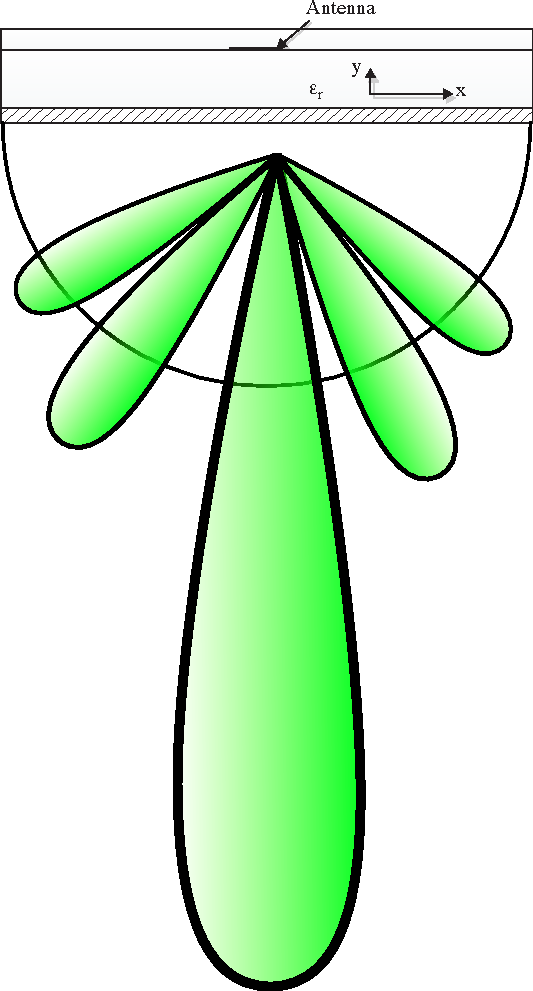
\includegraphics[width=.55\textwidth]{lens_onchipantennas.pdf}
                \label{fig:lens_on_chip}
            \end{figure}
        \end{column}
    \end{columns}
\end{frame}

\begin{frame}
    \frametitle{On-chip Antennas - Substrate Loss}
    \begin{columns}
        \begin{column}{.5\textwidth}
            \begin{outline}
                \1 The presence of metal vias
                \1 Lower permittivity substrates should be used to avoid the generation of surface waves.
                \1 Most of the waves actually get trapped and therefore attenuated to the low critical angle of \ch{Si} ($\arcsin 1/\sqrt{\E_{r,sub}}$)
            \end{outline}
        \end{column}
        \begin{column}{.5\textwidth}
            \begin{figure}[]
                \centering
                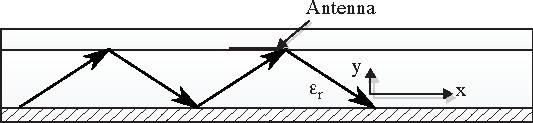
\includegraphics[width=1\textwidth]{surface_waves_onchipantennas.pdf}
                \label{fig:meta_vias}
            \end{figure}
        \end{column}
    \end{columns}
\end{frame}

\begin{frame}
    \frametitle{Class Activity}

    Alice is an antenna designer and needs to decide the best material as well as the topology of the antenna that will be \textit{integrated} with a CMOS circuit. The current design is giving her a poor radiation efficiency of \SI{30}{\percent}. Suggest some improvements to increase the antenna performance.

    \begin{figure}[h!]
        \centering
        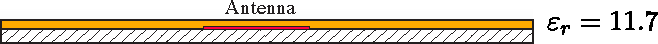
\includegraphics[width=.75\textwidth]{exercise.pdf}
    \end{figure}
\end{frame}

% \begin{frame}
%     \frametitle{Class Activity - Solution}

%     \begin{figure}
%         \centering
%         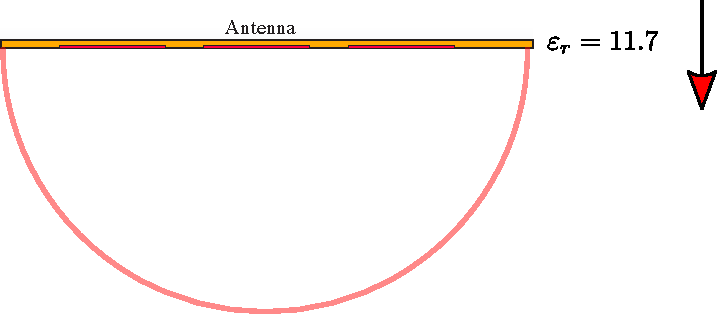
\includegraphics[width=.75\textwidth]{exercise_solution.pdf}
%     \end{figure}
% \end{frame}


\begin{frame}
    \frametitle{In-package Antennas}
    \begin{outline}
        \1 An in-package antenna consists of several co-planar metal layers
        \1 It is manufactured using a packaging process
        \1 Connections within the layers are made through vias
        \1 Due to better isolation, we can get better antenna performance compared to on-chip antennas
        \1 Antenna is created through an air cavity
        \1 Design requires a careful selection of permittivity of the substrate
        \1 Scaled microwave designs are used to fabricate antennas
    \end{outline}
    \begin{figure}[htbp]
        \centering
        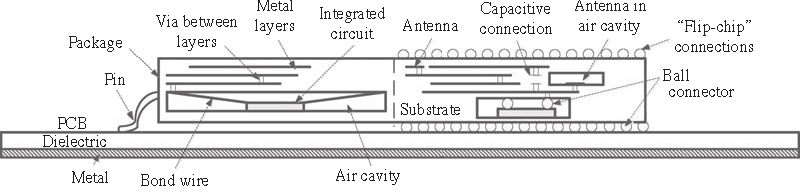
\includegraphics[width=.75\textwidth]{inpackage.pdf}
    \end{figure}
\end{frame}

\section{Beamforming Algorithms}

\begin{frame}
    \frametitle{Beamforming Algorithms}
    \begin{columns}[T]
        \begin{column}{.5\textwidth}
            \begin{outline}
                \small
                \1 For beamforming, determining the direction of an incoming signal through the direction of arrival (DoA) algorithms is a key element.
                \1 The goal is to develop a machine like the human ear
                \1 DoA or direction finding algorithms \textit{reconstruct} the signals from each direction and try to determine the identity of the signal source.
            \end{outline}
            \begin{align*}
                \small
                S_{i}=\sum_{\ell=1}^{N} m_{\ell}(t) e^{-j \overrightarrow{k_{\ell}} \cdot\left(\overrightarrow{r_{i}}-\overrightarrow{r_{1}}\right)}
            \end{align*}
            \tiny here $\overrightarrow{k_{\ell}}$ is the wave-vector, $\overrightarrow{r_{1}}$ and $\overrightarrow{r_{i}}$ are the positions of the reference and i-th array elements.
        \end{column}
        \begin{column}{.5\textwidth}
            \begin{figure}[T!]
                \centering
                \subfloat[]{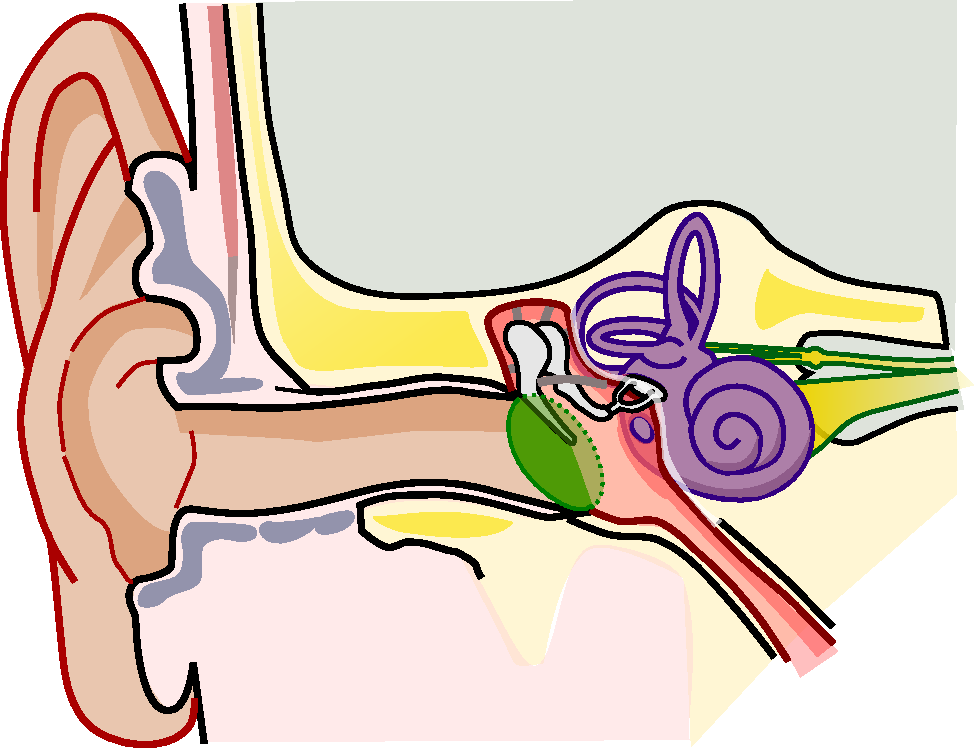
\includegraphics[width=.5\textwidth]{Anatomy_of_the_Human_Ear_blank.pdf}
                    \label{fig:antenna_on_chip}} \\
                \subfloat[]{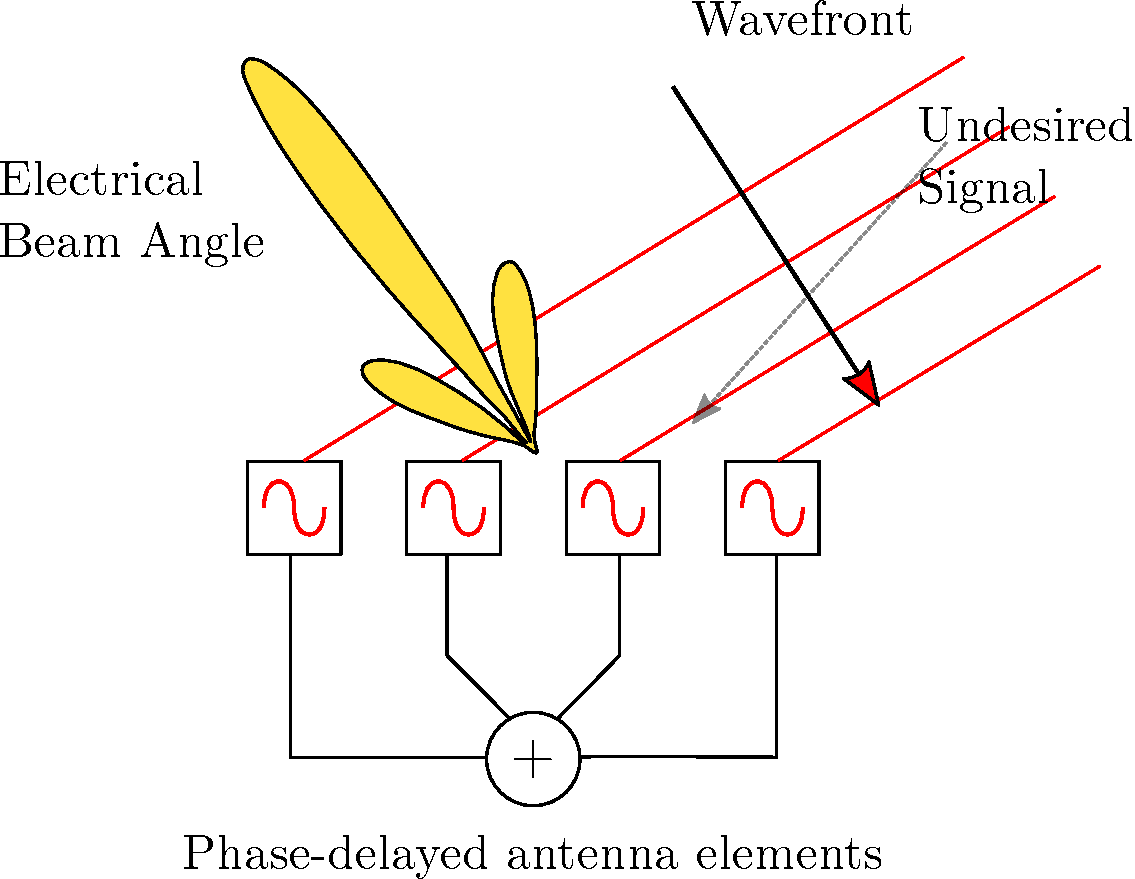
\includegraphics[width=.75\textwidth]{antenna_array_beamforming.pdf}
                    \label{fig:on_chip}}
            \end{figure}
        \end{column}
    \end{columns}
\end{frame}

\begin{frame}
    \frametitle{AoA Estimation}
    We seek to construct a matrix, $\mathbf{X}$ for an array of $M$ elements with $N$ snapshots recorded in time.
    \begin{align*}
        \mathbf{X}=\left[\begin{array}{ccc}
                S_{1}\left(t_{1}\right) & \ldots & S_{1}\left(t_{N}\right) \\
                \ldots                  & \ldots & \ldots                  \\
                S_{M}\left(t_{1}\right) & \ldots & S_{M}\left(t_{N}\right)
            \end{array}\right]
    \end{align*}
    Next, a covariance matrix $\mathbf{R}$ needs to be estimated for the incoming signal $\mathbf{X}$ polluted with noise $N$,
    \begin{align*}
        \mathbf{R}=\left(\frac{1}{N}\right) \mathbf{X}^{*} \mathbf{X}
    \end{align*}
    We also need to \textit{track} the directions in which the array is activated. We represent this with a steering vector,
    \begin{align*}
        \mathbf{a}_{\text {direction }}=\left[\begin{array}{llll}
                1 & e^{-j \overrightarrow{k_{l}} \cdot\left(\overrightarrow{r_{1}}-\overrightarrow{r_{2}}\right)} & \ldots & e^{-j \overrightarrow{k_{l}} \cdot\left(\overrightarrow{r_{1}}-r \vec{M}\right)}
            \end{array}\right]
    \end{align*}
\end{frame}

\begin{frame}
    \frametitle{AoA Estimation Contd.}

    The next step involves the intensive computation of weights which will be applied to each direction vector:
    \begin{align*}
        \mathbf{w}=\frac{\mathbf{R}^{-1} \mathbf{a}_{\text {direction }}}{\left(\mathbf{a}_{\text {direction }}^{*} \mathbf{R}^{-1} \mathbf{a}_{\text {direction }}\right)}
    \end{align*}

    \begin{outline}
        \1 There are established ways to solve the above matrices
        \1 Two of the most famous direction-finding algorithms are  multiple signal classification (MUSIC) and estimation of signal parameters via rotational invariance techniques (ESPIRIT)
        \1 Using some terminologies from Linear Algebra, both the algorithms above assume the covariance matrix column space is spanned by two orthogonal subspaces
        \2 They are signal and noise subspaces
    \end{outline}

\end{frame}

\begin{frame}
    \frametitle{DoA Output}

    \begin{figure}[h!]
        \centering
        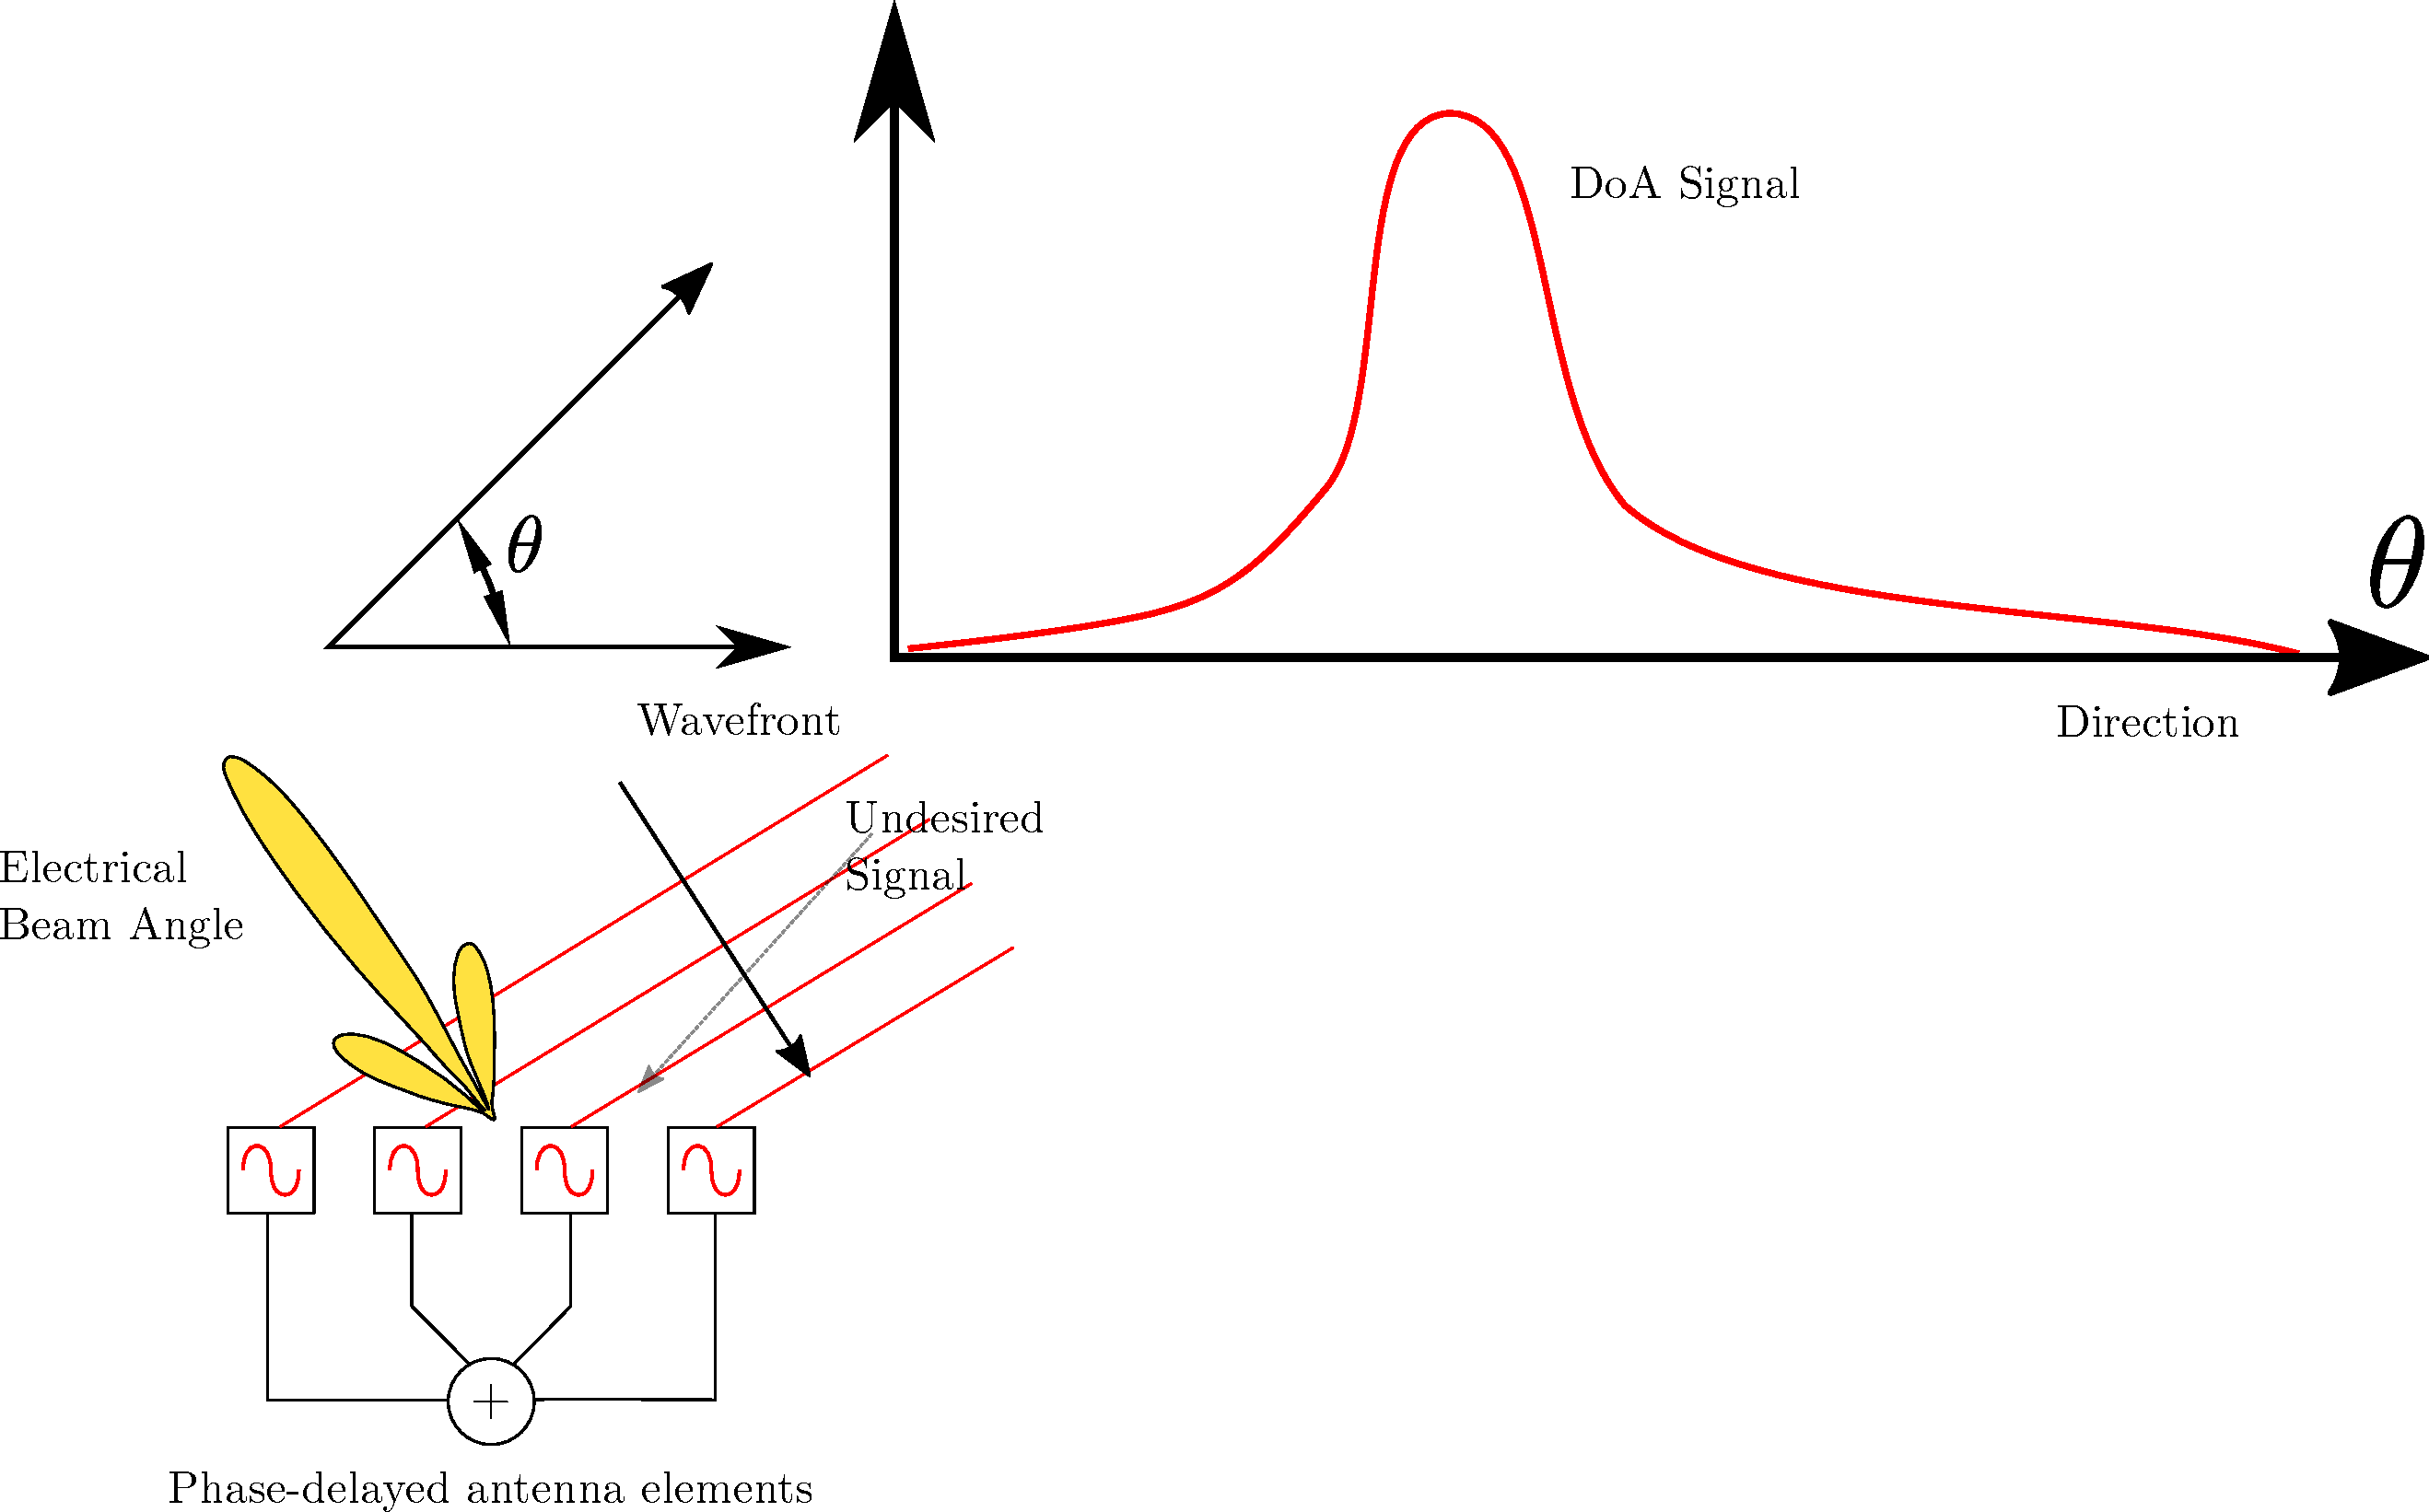
\includegraphics[width=.7\textwidth]{DoA.pdf}
    \end{figure}
\end{frame}

\begin{frame}
    \frametitle{Take home Messages}
    \begin{outline}
        \1 Going up in frequency not always results in higher channel capacity
        \1 mmWave Channel constrants can be overcome by high-gain, antenna arrays
        \1 For mmWave networks, maintaining a practical link budget requires beamforming
        \1 mmWave antenna is a hot research topic
        \1 High antenna efficiency
    \end{outline}
\end{frame}

\begin{frame}
    \frametitle{Further Reading}

    Chapter 4

    T. S. Rappaport, R. W. Heath, R. C. Daniels, and J. N. Murdock, Millimeter wave wireless communications. Upper Saddle River, NJ: Prentice Hall, 2015.

\end{frame}
\end{document}
